\documentclass[12pt]{article}

\usepackage{sbc-template}
\usepackage{graphicx,url}
\usepackage[utf8]{inputenc}
\usepackage[brazil]{babel}
\usepackage[latin1]{inputenc}  

     
\sloppy

\title{Do Caos ao Conhecimento: Uma Abordagem Baseada em RAG para Análise de Causa Raiz em Microsserviços}

\author{Daniel F. Schulz\inst{1}, Fabio Kon\inst{1}}


\address{Instituto de Matemática e Estatística -- Universidade de São Paulo
  (USP)
  \email{danielschulz@usp.br, kon@ime.usp.br}
}

\begin{document} 

\maketitle

\begin{abstract}
  This meta-paper describes the style to be used in articles and short papers
  for SBC conferences. For papers in English, you should add just an abstract
  while for the papers in Portuguese, we also ask for an abstract in
  Portuguese (``resumo''). In both cases, abstracts should not have more than
  10 lines and must be in the first page of the paper.
\end{abstract}
     
\begin{resumo} 
  Este meta-artigo descreve o estilo a ser usado na confecção de artigos e
  resumos de artigos para publicação nos anais das conferências organizadas
  pela SBC. É solicitada a escrita de resumo e abstract apenas para os artigos
  escritos em português. Artigos em inglês deverão apresentar apenas abstract.
  Nos dois casos, o autor deve tomar cuidado para que o resumo (e o abstract)
  não ultrapassem 10 linhas cada, sendo que ambos devem estar na primeira
  página do artigo.
\end{resumo}


\section{Introdução}



\section{Referencial Teórico} \label{sec:firstpage}



\section{Trabalhos Relacionados}


\section{Proposta}

Esta seção apresenta uma metodologia para construir e utilizar conhecimento
diagnóstico em aplicações de microsserviços. O conhecimento é gerado a partir
de experimentos de injeção de falhas e organizado em pares de documentos: um
descreve os sintomas observados e o outro registra um guia de investigação.
Em uma nova ocorrência, os guias recuperados orientam verificações adicionais,
enquanto o diagnóstico se apoia nas evidências coletadas para o caso atual.
A Figura~\ref{fig:arquitetura} resume as duas fases da metodologia.

\subsection{Visão Geral da Arquitetura}

A metodologia compreende duas fases: geração do conhecimento e diagnóstico
assistido. Na primeira, experimentos de injeção de falhas produzem dados de
telemetria usados para construir pares de documentos A/B. O documento A
descreve os sinais observados, enquanto o documento B registra um guia de
investigação associado ao experimento. Os pares aprovados pelos critérios de
elegibilidade ficam disponíveis para recuperação.

Na segunda fase, uma nova ocorrência é analisada a partir de sua telemetria.
A descrição inicial dos sintomas é usada para recuperar documentos A de
experimentos históricos e seus respectivos guias B. Esses guias orientam a
formulação de hipóteses e a seleção de consultas adicionais às fontes de
telemetria. Os resultados das consultas realizadas no caso atual fundamentam
a elaboração do diagnóstico.

\begin{figure}[ht]
\centering
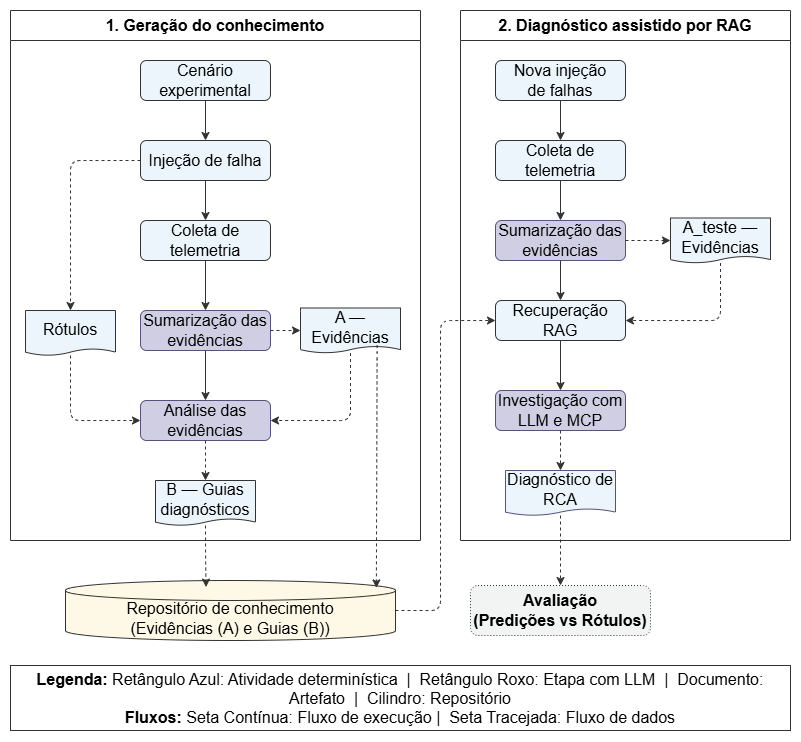
\includegraphics[width=.9\textwidth]{Fluxo_artigo.png}
\caption{Arquitetura da metodologia de geração e utilização de conhecimento
diagnóstico.}
\label{fig:arquitetura}
\end{figure}

Na versão avaliada, o modelo de linguagem Qwen 3.5 é utilizado na produção
dos documentos, na proposição de verificações e na elaboração do diagnóstico.
A recuperação é realizada pelo mecanismo de busca descrito na
Seção~\ref{sec:recuperacao}. O conhecimento é armazenado externamente, sem
ajuste dos parâmetros do modelo. O acesso às fontes de telemetria ocorre por
meio de ferramentas disponibilizadas pelo \textit{Model Context Protocol}
(MCP).

\subsection{Modelo do Sistema e Representação do Conhecimento}

Considera-se uma aplicação composta por um conjunto de microsserviços
$V=\{v_1,\ldots,v_n\}$ e sujeita a tipos de falha pertencentes a
$F=\{f_1,\ldots,f_m\}$. Entre os tipos considerados estão sobrecarga de CPU,
consumo elevado de memória, latência de rede, erros HTTP e interrupção de
contêineres.

Cada experimento $j$ injeta uma falha $f_j^*\in F$ em um serviço-alvo
$s_j^*\in V$. Durante sua execução, coleta-se a telemetria
$T_j=\langle M_j,L_j,R_j\rangle$, composta por métricas, \textit{logs} e
rastros distribuídos (\textit{traces}). Esses dados são associados aos
períodos de referência e de ocorrência da falha.

O conhecimento diagnóstico é representado por pares de documentos
$(D_{A,j},D_{B,j})$:

\begin{itemize}
  \item \textbf{Documento A -- Descrição dos sintomas:}
  $D_{A,j}=\psi(T_j)$ caracteriza os sinais observados na telemetria sem
  receber os rótulos $(s_j^*,f_j^*)$ do experimento;

  \item \textbf{Documento B -- Guia de investigação:}
  $D_{B,j}=\Phi(D_{A,j},T_j,s_j^*,f_j^*)$ registra as hipóteses investigadas,
  as consultas realizadas, seus resultados e as referências às evidências
  relacionadas ao diagnóstico.
\end{itemize}

Seja $\mathcal{J}$ o conjunto de experimentos para os quais foram produzidos
pares A/B. A base completa é representada por:

\begin{equation}
  \mathcal{B} =
  \{(D_{A,j},D_{B,j}) \mid j\in\mathcal{J}\}.
\end{equation}

Uma função de elegibilidade $Q(j)$ verifica o guia do experimento $j$,
considerando seus rótulos, as evidências coletadas e o resultado da revisão
do guia. O conjunto disponibilizado para recuperação é:

\begin{equation}
  \mathcal{K} =
  \{(D_{A,j},D_{B,j}) \mid j\in\mathcal{J},\ Q(j)=1\}.
\end{equation}

\subsection{Geração do Conhecimento Diagnóstico}

A geração começa com experimentos de injeção de falhas, nos quais são
registrados o serviço-alvo, o tipo de falha e os períodos de referência e de
ocorrência da falha. Esses períodos orientam as consultas às fontes de
telemetria.

A partir das evidências iniciais, o modelo produz o documento A, que descreve
os sinais observados, como variações de métricas, padrões em \textit{logs},
informações de rastros e relações entre serviços. Os rótulos do experimento
não são fornecidos nessa etapa.

Em seguida, o modelo produz o documento B com base em A, nas evidências
coletadas e nos rótulos do experimento. Os rótulos orientam a construção do
guia, que reúne hipóteses, passos de investigação, resultados observados,
verificações recomendadas e limitações.

Os pares A/B são armazenados com suas informações de origem e submetidos a
verificações de formato e integridade das referências, além dos critérios de
elegibilidade. Entre esses critérios estão a correspondência entre o
diagnóstico e os rótulos do experimento, o registro dos resultados das
consultas e a referência às evidências, incluindo um sinal compatível com a
falha no serviço-alvo. A elegibilidade também considera uma revisão
automatizada do guia, realizada pelo próprio modelo, que avalia a
correspondência entre o diagnóstico, os rótulos e as evidências
referenciadas. Essa revisão não constitui uma validação independente.
Apenas os pares aprovados ficam disponíveis para recuperação.

\subsection{Recuperação de Guias de Investigação}
\label{sec:recuperacao}

Em uma nova ocorrência $c$, a telemetria coletada é usada para produzir uma
descrição inicial dos sintomas, $D_{A,c}=\psi(T_c)$. A recuperação seleciona
pares históricos elegíveis relacionados a essa descrição:

\begin{equation}
  \mathcal{R}_c =
  \operatorname{Retrieve}(D_{A,c},\mathcal{K}),
  \qquad \mathcal{R}_c\subseteq\mathcal{K}.
\end{equation}

Na versão avaliada, a busca compara a descrição atual com os documentos A dos
experimentos históricos por dois caminhos. O primeiro ordena os documentos
pela correspondência entre termos, usando BM25. O segundo compara os aumentos
de métricas por serviço entre os períodos de referência e de ocorrência da
falha. Para cada métrica, os aumentos são ajustados pela mediana das
variações absolutas não nulas observadas nos documentos históricos.

Quando um aumento ajustado atinge o limiar configurado, os ordenamentos por
termos e por métricas são combinados; caso contrário, utiliza-se apenas o
ordenamento por termos. Os parâmetros dessa combinação são descritos na
seção de avaliação experimental. Na comparação numérica, valores ausentes
são representados por zero, o que pode aproximar a falta de uma medição da
ausência de variação.

A busca seleciona até três pares elegíveis. O limite de tamanho do contexto
pode reduzir a quantidade de guias B enviada ao modelo. Os guias recuperados
indicam possibilidades de investigação, não respostas para o caso atual.
Se nenhum guia for recuperado, a investigação pode prosseguir com as
evidências disponíveis.

\subsection{Diagnóstico Assistido por Conhecimento Histórico}

O procedimento de diagnóstico utiliza a descrição A do caso atual, os guias
selecionados entre os pares recuperados e as evidências já coletadas. De
forma abstrata, a estimativa de serviço e tipo de falha é representada por:

\begin{equation}
  (\hat{s},\hat{f}) =
  \Gamma(D_{A,c},\mathcal{R}_c,\mathcal{P}_{\text{MCP}}),
\end{equation}

em que $\Gamma$ representa o procedimento de diagnóstico assistido,
$\hat{s}$ e $\hat{f}$ são o serviço e o tipo de falha estimados, e
$\mathcal{P}_{\text{MCP}}$ representa as ferramentas de consulta às fontes
de telemetria.

Com essas informações, o modelo propõe hipóteses e verificações adicionais.
Por exemplo, diante de um aumento de latência em um serviço, um guia pode
orientar a comparação entre o uso de CPU desse serviço e a latência das
chamadas às suas dependências.

As verificações propostas são avaliadas pelo executor e, quando aceitas,
realizadas por meio das ferramentas MCP. O modelo recebe os resultados e
pode propor novas consultas ou encerrar a investigação, de acordo com os
limites configurados. Os guias históricos orientam a investigação, mas as
conclusões se apoiam nas evidências do incidente atual.

Ao final, o modelo produz um diagnóstico com o serviço e o tipo de falha
estimados como causa raiz, as evidências de suporte, as hipóteses alternativas
e as limitações da análise. O Algoritmo~\ref{alg:metodologia} resume as etapas
de geração e uso do conhecimento.





\subsection{Subsections}



\section{Avaliação Experimental}


\section{Conclusão e Trabalhos Futuros}

Figure and table captions should be centered if less than one line
(Figure~\ref{fig:exampleFig1}), otherwise justified and indented by 0.8cm on
both margins, as shown in Figure~\ref{fig:exampleFig2}. The caption font must
be Helvetica, 10 point, boldface, with 6 points of space before and after each
caption.



\begin{figure}[ht]
\centering
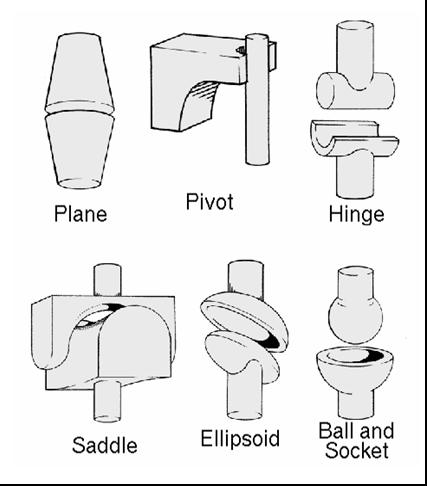
\includegraphics[width=.3\textwidth]{fig2.jpg}
\caption{This figure is an example of a figure caption taking more than one
  line and justified considering margins mentioned in Section~\ref{sec:figs}.}
\label{fig:exampleFig2}
\end{figure}

In tables, try to avoid the use of colored or shaded backgrounds, and avoid
thick, doubled, or unnecessary framing lines. When reporting empirical data,
do not use more decimal digits than warranted by their precision and
reproducibility. Table caption must be placed before the table (see Table 1)
and the font used must also be Helvetica, 10 point, boldface, with 6 points of
space before and after each caption.

\begin{table}[ht]
\centering
\caption{Variables to be considered on the evaluation of interaction
  techniques}
\label{tab:exTable1}
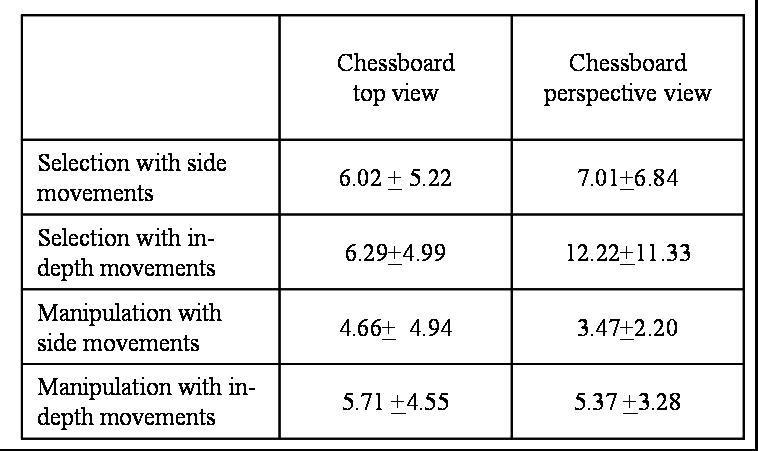
\includegraphics[width=.7\textwidth]{table.jpg}
\end{table}

\section{Images}

All images and illustrations should be in black-and-white, or gray tones,
excepting for the papers that will be electronically available (on CD-ROMs,
internet, etc.). The image resolution on paper should be about 600 dpi for
black-and-white images, and 150-300 dpi for grayscale images.  Do not include
images with excessive resolution, as they may take hours to print, without any
visible difference in the result. 

\section{References}

Bibliographic references must be unambiguous and uniform.  We recommend giving
the author names references in brackets, e.g. \cite{knuth:84},
\cite{boulic:91}, and \cite{smith:99}.

The references must be listed using 12 point font size, with 6 points of space
before each reference. The first line of each reference should not be
indented, while the subsequent should be indented by 0.5 cm.

\bibliographystyle{sbc}
\bibliography{sbc-template}

\end{document}
